\chapter{系统启动与初始化}

我将本系统的启动与初始化分为三个阶段:

\begin{itemize}
    \item \textbf{QEMU初始化}
    \item \textbf{引导程序}
    \item \textbf{内核初始化}
\end{itemize}

\section{QEMU初始化}

这个阶段在真实计算机的启动中是加载ROM的过程。机器上电、文件加载到内存后,QEMU CPU的PC会被设置为0x1000,然后执行第一阶段的代码。
它会对CPU进行一些初始化操作,然后把控制权移交给bootloader,它的跳转地址固定是0x80000000处,我的BootLoader(rustsbi-qemu.bin)被预先加载到这里。

\section{引导程序}

在实际计算机中,Loader会进行内存初始化,并加载Runtime和BootLoader。BootLoader会进行硬件初始化和OS镜像的加载,而Runtime为OS提供运行时服务,
它是对硬件最基础的抽象,\href{https://github.com/riscv-non-isa/riscv-sbi-doc}{SBI}
就是RISC-V架构下的Runtime规范。

不过在NimlothOS中,引导程序和os镜像均在QEMU初始化阶段便已经被加载到了内存中,地址跳转以后直接进入rustsbi-qemu.bin程序,它会初始化硬件并提供SBI服务。

RustSBI的初始化结束以后,会跳转到预设好的0x80200000,这里放有内核镜像。

\section{内核初始化}

第三阶段是内核控制下操作系统各个模块的初始化,内核的入口函数是\lstinline[language=Rust]{rust_main},
它会在内核初始化完成后进入主循环调度。

\begin{lstlisting}[language=Rust,caption={内核初始化}, label={lst:kernel-init}]
#[unsafe(no_mangle)]
pub fn rust_main() -> ! {
    clear_bss();
    log::init();
    ::log::info!("[kernel] Hello, world!");
    mm::init();
    trap::init();
    trap::enable_timer_interrupt();
    timer::next_trigger();
    fs::list_apps();
    process::add_initproc();
    process::run_process();

    panic!("Unreachable in rust_main!");
}
\end{lstlisting}

下面进行详细介绍。

\subsection{内核镜像的内存分布}

默认链接器的内存布局是独立地址空间,但需要通过linker-qemu.ld脚本指定以符合QEMU的内存布局。调整后的具体布局如下:

\begin{figure}[htbp]
    \centering
    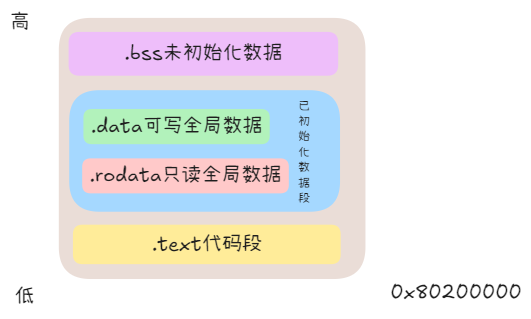
\includegraphics[width=0.6\textwidth]{../image/内核ELF布局.png}
    \caption{内核ELF布局}
    \label{fig:kernel-elf}
\end{figure}

通过 \texttt{rust-objdump} 工具查看编译后的内核镜像的各段分布与大小如下:

\begin{lstlisting}[language=Plain,caption={内核段分布信息}, label={lst:kernel-layout}]
$ rust-objdump -h target/riscv64gc-unknown-none-elf/release/os
target/riscv64gc-unknown-none-elf/release/os:   file format elf64-littleriscv
Sections:
Idx Name              Size     VMA              Type
1   .text             000178d0 0000000080200000 TEXT
2   .rodata           00005988 0000000080218000 DATA
3   .data             00000010 000000008021e000 DATA
4   .bss              00310330 000000008021f000 BSS
\end{lstlisting}

\subsection{汇编入口}

内核启动时的真正入口是一段汇编代码。在此之前,entry.asm会进行一些准备工作。它定义了内核入口函数\lstinline[language=Rust]{_start},
并把它放到.text的最低处(也即0x80200000处),另外在bss段建立大小64KB的内核启动栈。

运行时,\lstinline[language=Rust]{_start}会设置栈指针sp到栈顶并调用\lstinline[language=Rust]{rust_main},
然后过渡到\lstinline[language=Rust]{rust_main}代码中按顺序进行初始化。

\subsection{BSS段清零}

BSS段保护程序中未初始化的全局变量和静态变量,在程序加载过程中,它们需要被初始化为零。NimlothOS会利用链接文件里的符号sbss和ebss对这段
进行逐字节的清理。

\begin{lstlisting}[language=Rust,caption={bss段清零}, label={lst:bss-clear}]
fn clear_bss() {
    unsafe extern "C" {
        fn sbss();
        fn ebss();
    }
    unsafe {
        core::slice::from_raw_parts_mut(sbss as usize as *mut u8, ebss as usize - sbss as usize)
            .fill(0);
    }
}
\end{lstlisting}

\subsection{日志系统初始化}
日志系统在开发初期内置于内核中,现在正在尝试通过后期实现的管道机制将它从内核中抽离出来。内核中的日志系统基于Rust的log库实现
了Log trait,它的初始化工作是注册全局记录器并设置日志级别。

\subsection{内存系统初始化}
内存系统初始化的任务是按正确的顺序初始化内存管理的各个组件,确保系统能正常地进行内存分配和虚拟地址转化。
它会依次进行堆分配器初始化,物理页帧分配器初始化,并启用虚拟内存管理。

\begin{lstlisting}[language=Rust,caption={内存系统初始化}, label={lst:memory-init}]
pub fn init() {
    heap_allocator::init_heap();
    frame_allocator::init_frame_allocator();
    KERNEL_SPACE.exclusive_access().activate();
}
\end{lstlisting}

首先需要进行堆分配器的初始化,将静态分配的内核堆空间注册到堆分配器中,以便其可以用于动态内存分配。
这块空间位于前面提到的.bss段中,会一起被清零。

\begin{lstlisting}[language=Rust,caption={内核堆空间}, label={lst:heap-space}]
static mut HEAP_SPACE: [u8; KERNEL_HEAP_SIZE] = [0; KERNEL_HEAP_SIZE];
\end{lstlisting}

然后进行全局页帧分配器的初始化,设置它可用的物理内存范围。这里使用链接器脚本中定义的内核镜像的结束位置ekernel
作为可用物理内存的起点,终点通过硬编码到0x81000000,这样从0x80000000开始,可使用内存的整体大小为16MB。

\begin{lstlisting}[language=Rust,caption={物理页帧分配器初始化}, label={lst:frame-allocator-init}]
pub const MEMORY_END: usize = 0x8100_0000;

pub fn init_frame_allocator() {
    unsafe extern "C" {
        fn ekernel();
    }
    FRAME_ALLOCATOR.exclusive_access().init(
        PhysAddr::from(ekernel as usize).ceil(),
        PhysAddr::from(MEMORY_END).floor(),
    );
}
\end{lstlisting}

init会初始化一个简单的栈式页帧分配器StackFrameAllocator,其中的ceil和floor分别向上对齐和向下对齐到页边界。

最后,创建内核地址空间,并修改satp寄存器的值,启用SV39分页模式。我们的内核地址空间与xv6一样使用恒等映射,这样在
地址转化激活前后可以最大程度减少工作量。

\begin{lstlisting}[language=Rust,caption={内核地址空间激活}, label={lst:kernel-space-activate}]
pub fn activate(&self) {
    let satp = self.page_table.token();
    unsafe {
        satp::write(satp);
        asm!("sfence.vma");
    }
}
\end{lstlisting}

token函数根据页表的根节点计算出satp寄存器的值,然后通过asm!宏调用汇编指令写入satp寄存器,并执行sfence.vma指令,
刷新TLB缓存。

\begin{lstlisting}[language=Rust,caption={内核地址空间初始化}, label={lst:kernel-space-init}]
pub fn new_kernel() -> Self {
    let mut memory_set = Self::new_bare();
    memory_set.map_trampoline();
    println!(".text [{:#x}, {:#x})", stext as usize, etext as usize);
    println!(".rodata [{:#x}, {:#x})", srodata as usize, erodata as usize);
    println!(".data [{:#x}, {:#x})", sdata as usize, edata as usize);
    println!(
        ".bss [{:#x}, {:#x})",
        sbss_with_stack as usize, ebss as usize
    );
    println!("mapping .text section");
    memory_set.push(
        MapArea::new(
            (stext as usize).into(),
            (etext as usize).into(),
            MapType::Identical,
            MapPermission::R | MapPermission::X,
        ),
        None,
    );
    println!("mapping .rodata section");
    memory_set.push(
        MapArea::new(
            (srodata as usize).into(),
            (erodata as usize).into(),
            MapType::Identical,
            MapPermission::R,
        ),
        None,
    );
    println!("mapping .data section");
    memory_set.push(
        MapArea::new(
            (sdata as usize).into(),
            (edata as usize).into(),
            MapType::Identical,
            MapPermission::R | MapPermission::W,
        ),
        None,
    );
    println!("mapping .bss section");
    memory_set.push(
        MapArea::new(
            (sbss_with_stack as usize).into(),
            (ebss as usize).into(),
            MapType::Identical,
            MapPermission::R | MapPermission::W,
        ),
        None,
    );
    println!("mapping physical memory");
    memory_set.push(
        MapArea::new(
            (ekernel as usize).into(),
            MEMORY_END.into(),
            MapType::Identical,
            MapPermission::R | MapPermission::W,
        ),
        None,
    );
    println!("mapping memory-mapped registers");
    for pair in MMIO {
        memory_set.push(
            MapArea::new(
                (*pair).0.into(),
                ((*pair).0 + (*pair).1).into(),
                MapType::Identical,
                MapPermission::R | MapPermission::W,
            ),
            None,
        );
    }
    memory_set
}
\end{lstlisting}

\subsection{陷阱处理系统初始化与时钟中断设置}

陷阱处理系统与任务调度、信号处理等模块都有关,它的初始化只需要设置内核态陷阱入口,
用户态陷阱入口会在任务切换时的trap\_return中调用。内核态陷阱指向处理函数trap\_from\_kernel,
该函数输出陷阱相关寄存器后直接panic。

\begin{lstlisting}[language=Rust,caption={陷阱处理系统初始化与时钟中断设置}, label={lst:trap-timer-init}]
pub fn init() {
    set_kernel_trap_entry();
    enable_timer_interrupt();
}

pub fn next_trigger() {
    timer(time() + CLOCK_FREQ / TICKS_PER_SEC);
}
\end{lstlisting}

然后init函数还会启用时钟中断,设置sie\.STIE位,允许时钟中断触发陷阱。定时器和时钟模块也会调用
next\_trigger函数设置下一次时钟中断的触发时间。这也是进程调度系统的基础。

\subsection{文件系统初始化}
文件系统会调用list\_apps函数,在这个过程中惰性初始化的静态变量ROOT\_INODE,BLOCK\_DEVICE都会
进行加载,并调用文件系统的open函数来读取挂载到VirtIO块设备上的文件,恢复磁盘上这个文件系统的状态。

\begin{lstlisting}[language=Rust,caption={文件系统初始化}, label={lst:filesystem-init}]
lazy_static! {
    pub static ref ROOT_INODE: Arc<Inode> = {
        let efs = EasyFileSystem::open(BLOCK_DEVICE.clone());
        Arc::new(EasyFileSystem::root_inode(&efs))
    };
    pub static ref BLOCK_DEVICE: Arc<dyn BlockDevice> = {
        let block_device = Arc::new(BlockDeviceImpl::new());
        block_device
    };
}
\end{lstlisting}

\subsection{进程管理系统初始化}

到这里前期的初始化工作就正式完成了,内核将会把初始进程加入到就绪队列中,这一过程中同样通过惰性初始化机制
创建全局任务管理器PROCESS\_MANAGER和pid映射表PID\_MAP。

\begin{lstlisting}[language=Rust,caption={进程管理系统初始化}, label={lst:process-manager-init}]
lazy_static!{
    pub static ref PROCESS_MANAGER: UPSafeCell<TaskManager> =
        unsafe { UPSafeCell::new(ProcessManager::new()) };
    pub static ref PID2TCB: UPSafeCell<BTreeMap<usize, Arc<ProcessControlBlock>>> =
        unsafe { UPSafeCell::new(BTreeMap::new()) };
}
\end{lstlisting}

initproc是一个特殊的进程,它的pid为1。作为第一个用户进程,它会启动用户态入口,通过fork和exec系统调用
加载user\_shell程序,进入用户命令行解释器。

\subsection{进入主循环调度}

进程的调度由系统的idle控制流完成,它运行在CPU核的启动栈上,永不返回,并且对于进程而言是透明的。
这一机制由run\_process和schedule函数合作实现。

在内核初始化完毕后,就会调用run\_process函数进入idle控制流。它会从全局进程管理器获取下一个待调度进程
并切换。进程主动调用yield系统调用退出或是本轮时间耗尽触发中断时,会调用schedule函数回到idle控制流中进行
下一步调度。

\begin{lstlisting}[language=Rust,caption={idle控制流}, label={lst:idle-control-flow}]
pub fn run_process() {
    loop {
        let mut processor = PROCESSOR.exclusive_access();
        if let Some(process) = fetch_process() {
            let idle_process_cx_ptr = processor.idle_process_cx_ptr();
            let mut process_inner = process.inner_exclusive_access();
            let next_process_cx_ptr = &process_inner.process_cx as *const ProcessContext;
            process_inner.process_status = ProcessStatus::Running;
            drop(process_inner);
            processor.current = Some(process);
            drop(processor);
            unsafe {
                __switch(idle_process_cx_ptr, next_process_cx_ptr);
            }
        }
    }
}

pub fn schedule(switched_process_cx_ptr: *mut ProcessContext) {
    let mut processor = PROCESSOR.exclusive_access();
    let idle_process_cx_ptr = processor.idle_process_cx_ptr();
    drop(processor);
    unsafe {
        __switch(switched_process_cx_ptr, idle_process_cx_ptr);
    }
}
\end{lstlisting}

至此,系统的启动与初始化过程就全部完成了,可以通过user\_shell输入来运行用户程序。

\begin{figure}[htbp]
    \centering
    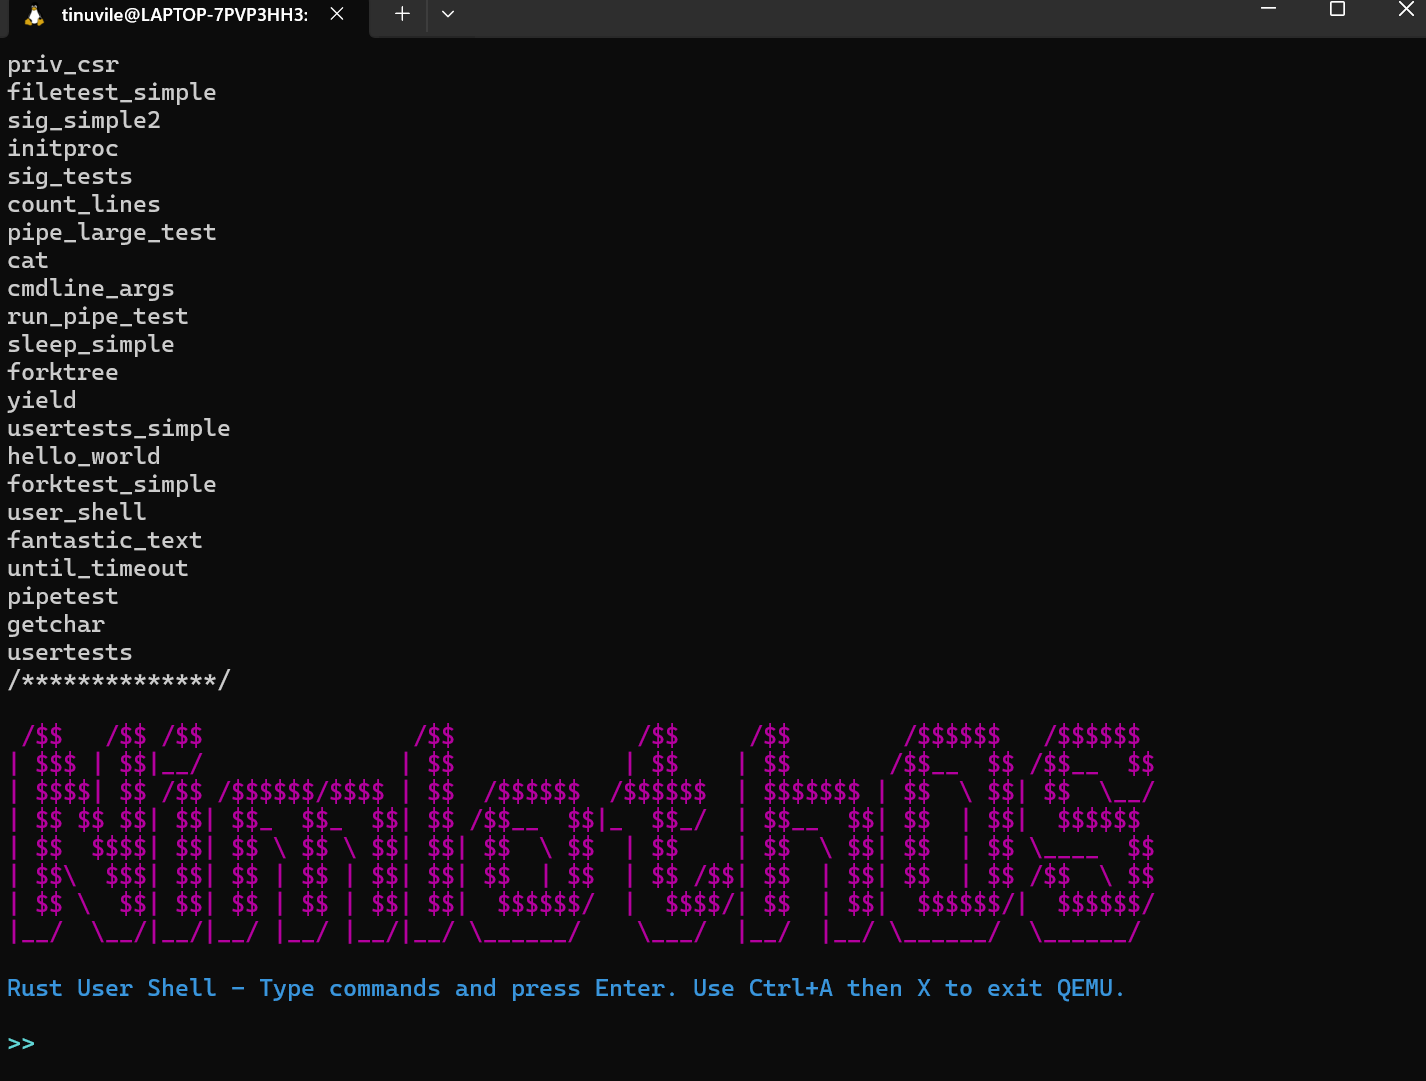
\includegraphics[width=0.6\textwidth]{../image/启动.png}
    \caption{启动}
    \label{fig:启动}
\end{figure}